\section{Experiment}
\begin{frame}{Experiment}
	
		BPR-MF\cite{rendle2009bpr} and CA-BPR\cite{DBLP:conf/webi/GuoWWT15}
	
	\begin{table}[htbp]
		\caption{Characteristics of compared methods}
		\renewcommand\arraystretch{1.3}%改变行高
		\label{tab:characteristic}
		\begin{center}
			\begin{tabular}{|c|c|c|}
				\hline
				Method   &   Content & Sampling \\
				\hline
				\renewcommand\arraystretch{1}%改变行高
				BPR-MF   &   no      & uniform  \\
				CA-BPR   &   yes     & non-uniform\\
				\hline
				
			\end{tabular}
		\end{center}
	\end{table}
\end{frame}

\begin{frame}{Experiment}
	\begin{table}[htbp]
		\caption{The performence of approaches by MAP and NDCG.}
		\label{tab:mapandndcg}
		\begin{center}
			\begin{tabular}{|c | c |c |c|c|c|}
				\hline
				BPR-MF  &   k=10 &   k=20 &    k=30&    k=40&    k=50\\
				\hline
				MAP      &  0.0879&  0.0877&  0.1043&  0.0888&  0.1074\\
				\hline
				NDCG@3   &  0.3051&  0.3545&  0.3398&  0.2491&  0.3790\\
				NDCG@5   &  0.3616&  0.4296&  0.3708&  0.2984&  0.4153\\
				NDCG@10  &  0.4120&  0.4632&  0.4010&  0.3163&  0.4458\\
				NDCG@20  &  0.4121&  0.4575&  0.4164&  0.3415&  0.4323\\
				\hline
			\end{tabular}
		\end{center}
	\end{table}
	
	\begin{table}
		
		\begin{center}
			
			\begin{tabular}{|c | c |c |c|c|c|}
				\hline
				CA-BPR  &     k=10&   k=20 &    k=30&  k=40 &   k=50  \\
				\hline
				MAP     &   0.1074&  0.1072&  0.1274&  0.1016&  0.1229\\
				\hline
				NDCG@3  &   0.3790&  0.4336&  0.4152&  0.3044&  0.4631\\
				NDCG@5  &   0.4153&  0.4752&  0.4531&  0.3646&  0.5074\\
				NDCG@10 &   0.4458&  0.5101&  0.4900&  0.3865&  0.5447\\
				NDCG@20 &   0.4323&  0.4946&  0.5088&  0.4173&  0.5282\\
				\hline
			\end{tabular}
		\end{center}
	\end{table}
\end{frame}

\begin{frame}{Experiment}
	\begin{figure}
		\begin{center}
			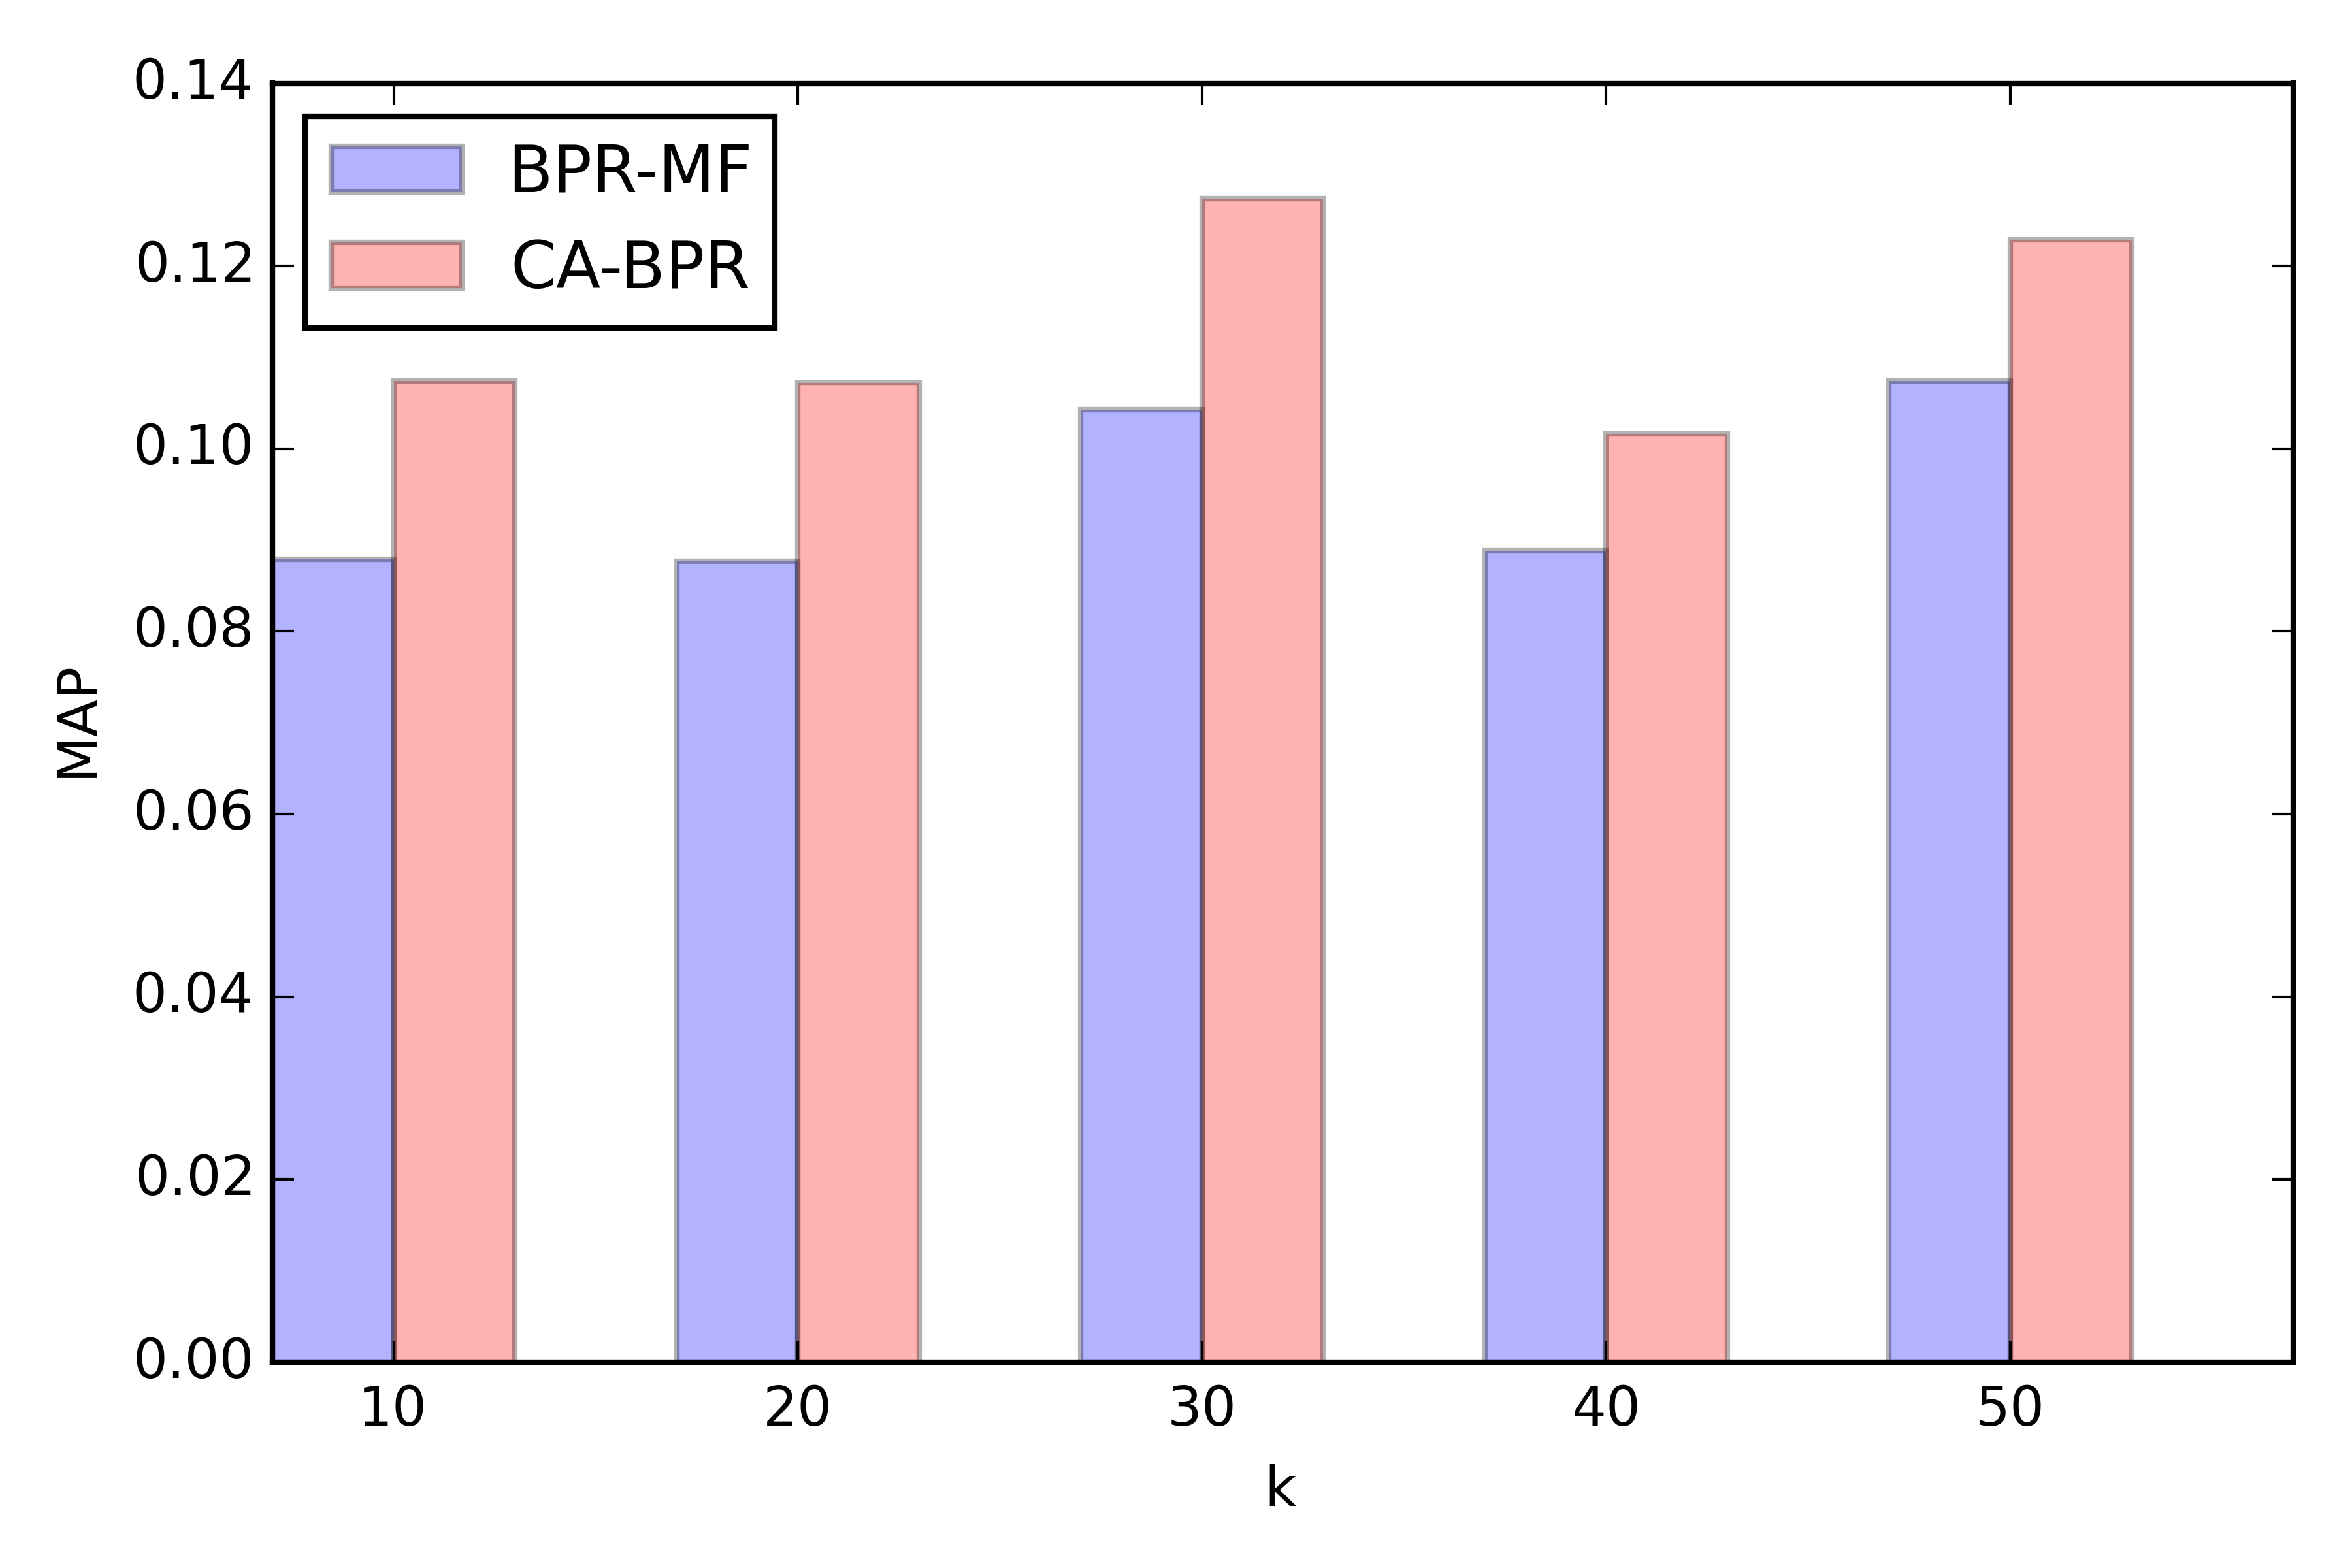
\includegraphics[width=3in]{bar}
		\end{center}
		\caption{CA-BPR indeed performs better than BPR-MF.}
	\end{figure}
\end{frame}

\begin{frame}
	\centering
	\Huge Thank you !
\end{frame}